\chapter{Ma trận}

\index{matrix}
\index{ma trận}

\key{Ma trận} (matrix) là một khái niệm toán học
tương ứng với mảng hai chiều
trong lập trình. Ví dụ,
\[
A = 
 \begin{bmatrix}
  6 & 13 & 7 & 4 \\
  7 & 0 & 8 & 2 \\
  9 & 5 & 4 & 18 \\
 \end{bmatrix}
\]
là một ma trận kích thước $3 \times 4$, tức là,
nó có 3 hàng và 4 cột.
Ký hiệu $[i,j]$ chỉ đến
phần tử ở hàng $i$ và cột $j$
trong ma trận.
Ví dụ, trong ma trận trên,
$A[2,3]=8$ và $A[3,1]=9$.

\index{vector}
\index{vectơ}

Một trường hợp đặc biệt của ma trận là \key{vectơ} (vector)
là ma trận một chiều kích thước $n \times 1$.
Ví dụ,
\[
V =
\begin{bmatrix}
4 \\
7 \\
5 \\
\end{bmatrix}
\]
là một vectơ chứa ba phần tử.

\index{transpose}
\index{chuyển vị}

\key{Chuyển vị} (transpose) $A^T$ của một ma trận $A$
được tạo ra khi các hàng và cột của $A$
được hoán đổi, tức là $A^T[i,j]=A[j,i]$:
\[
A^T = 
 \begin{bmatrix}
  6 & 7 & 9 \\
  13 & 0 & 5 \\
  7 & 8 & 4 \\
  4 & 2 & 18 \\
 \end{bmatrix}
\]

\index{square matrix}
\index{ma trận vuông}

Một ma trận là \key{ma trận vuông} (square matrix) nếu nó
có cùng số hàng và số cột.
Ví dụ, ma trận sau là một
ma trận vuông:

\[
S = 
 \begin{bmatrix}
  3 & 12 & 4  \\
  5 & 9 & 15  \\
  0 & 2 & 4 \\
 \end{bmatrix}
\]

\section{Các phép toán}

Tổng $A+B$ của các ma trận $A$ và $B$
được định nghĩa nếu các ma trận có cùng kích thước.
Kết quả là một ma trận trong đó mỗi phần tử
là tổng của các phần tử tương ứng
trong $A$ và $B$.

Ví dụ,
\[
 \begin{bmatrix}
  6 & 1 & 4 \\
  3 & 9 & 2 \\
 \end{bmatrix}
+
 \begin{bmatrix}
  4 & 9 & 3 \\
  8 & 1 & 3 \\
 \end{bmatrix}
=
 \begin{bmatrix}
  6+4 & 1+9 & 4+3 \\
  3+8 & 9+1 & 2+3 \\
 \end{bmatrix}
=
 \begin{bmatrix}
  10 & 10 & 7 \\
  11 & 10 & 5 \\
 \end{bmatrix}.
\]

Nhân một ma trận $A$ với một giá trị $x$ có nghĩa là
mỗi phần tử của $A$ được nhân với $x$.
Ví dụ,
\[
 2 \cdot \begin{bmatrix}
  6 & 1 & 4 \\
  3 & 9 & 2 \\
 \end{bmatrix}
=
 \begin{bmatrix}
  2 \cdot 6 & 2\cdot1 & 2\cdot4 \\
  2\cdot3 & 2\cdot9 & 2\cdot2 \\
 \end{bmatrix}
=
 \begin{bmatrix}
  12 & 2 & 8 \\
  6 & 18 & 4 \\
 \end{bmatrix}.
\]

\subsubsection{Phép nhân ma trận}

\index{matrix multiplication}
\index{phép nhân ma trận}

Tích $AB$ của các ma trận $A$ và $B$
được định nghĩa nếu $A$ có kích thước $a \times n$
và $B$ có kích thước $n \times b$, tức là,
chiều rộng của $A$ bằng chiều cao của $B$.
Kết quả là một ma trận kích thước $a \times b$
với các phần tử được tính bằng công thức
\[
AB[i,j] = \sum_{k=1}^n A[i,k] \cdot B[k,j].
\]

Ý tưởng là mỗi phần tử của $AB$
là một tổng các tích của các phần tử của $A$ và $B$
theo hình minh họa sau:

\begin{center}
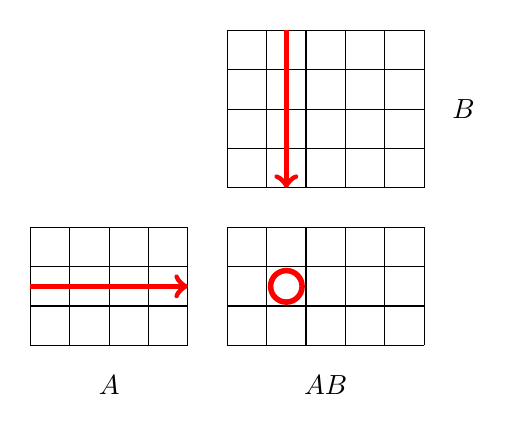
\begin{tikzpicture}[scale=0.5]
\draw (0,0) grid (4,3);
\draw (5,0) grid (10,3);
\draw (5,4) grid (10,8);

\node at (2,-1) {$A$};
\node at (7.5,-1) {$AB$};
\node at (11,6) {$B$};

\draw[thick,->,red,line width=2pt] (0,1.5) -- (4,1.5);
\draw[thick,->,red,line width=2pt] (6.5,8) -- (6.5,4);
\draw[thick,red,line width=2pt] (6.5,1.5) circle (0.4);
\end{tikzpicture}
\end{center}

Ví dụ,

\[
 \begin{bmatrix}
  1 & 4 \\
  3 & 9 \\
  8 & 6 \\
 \end{bmatrix}
\cdot
 \begin{bmatrix}
  1 & 6 \\
  2 & 9 \\
 \end{bmatrix}
=
 \begin{bmatrix}
  1 \cdot 1 + 4 \cdot 2 & 1 \cdot 6 + 4 \cdot 9 \\
  3 \cdot 1 + 9 \cdot 2 & 3 \cdot 6 + 9 \cdot 9 \\
  8 \cdot 1 + 6 \cdot 2 & 8 \cdot 6 + 6 \cdot 9 \\
 \end{bmatrix}
=
 \begin{bmatrix}
  9 & 42 \\
  21 & 99 \\
  20 & 102 \\
 \end{bmatrix}.
\]

Phép nhân ma trận có tính kết hợp,
tức là $A(BC)=(AB)C$ thỏa mãn,
nhưng không có tính giao hoán,
tức là thường thì $AB \neq BA$.

\index{identity matrix}
\index{ma trận đơn vị}

\key{Ma trận đơn vị} (identity matrix) là ma trận vuông
mà mỗi phần tử trên đường chéo là 1
và tất cả các phần tử khác là 0.
Ví dụ, ma trận sau
là ma trận đơn vị $3 \times 3$:
\[
 I = \begin{bmatrix}
  1 & 0 & 0 \\
  0 & 1 & 0 \\
  0 & 0 & 1 \\
 \end{bmatrix}
\]

\begin{samepage}
Nhân một ma trận với một ma trận đơn vị
không làm thay đổi nó. Ví dụ,
\[
 \begin{bmatrix}
  1 & 0 & 0 \\
  0 & 1 & 0 \\
  0 & 0 & 1 \\
 \end{bmatrix}
\cdot
 \begin{bmatrix}
  1 & 4 \\
  3 & 9 \\
  8 & 6 \\
 \end{bmatrix}
=
 \begin{bmatrix}
  1 & 4 \\
  3 & 9 \\
  8 & 6 \\
 \end{bmatrix} \hspace{10px} \textrm{và} \hspace{10px}
 \begin{bmatrix}
  1 & 4 \\
  3 & 9 \\
  8 & 6 \\
 \end{bmatrix}
\cdot
 \begin{bmatrix}
  1 & 0 \\
  0 & 1 \\
 \end{bmatrix}
=
 \begin{bmatrix}
  1 & 4 \\
  3 & 9 \\
  8 & 6 \\
 \end{bmatrix}.
\]
\end{samepage}

Sử dụng một thuật toán đơn giản,
ta có thể tính tích của
hai ma trận $n \times n$
trong thời gian $O(n^3)$.
Cũng có những thuật toán hiệu quả hơn
cho phép nhân ma trận\footnote{Thuật toán đầu tiên như vậy
là thuật toán Strassen,
được công bố năm 1969 \cite{str69},
có độ phức tạp thời gian là $O(n^{2.80735})$;
thuật toán tốt nhất hiện tại \cite{gal14}
chạy trong thời gian $O(n^{2.37286})$.},
nhưng chúng chủ yếu mang tính lý thuyết
và những thuật toán như vậy không cần thiết
trong lập trình thi đấu.


\subsubsection{Lũy thừa ma trận}

\index{matrix power}
\index{lũy thừa ma trận}

Lũy thừa $A^k$ của một ma trận $A$ được định nghĩa
nếu $A$ là ma trận vuông.
Định nghĩa dựa trên phép nhân ma trận:
\[ A^k = \underbrace{A \cdot A \cdot A \cdots A}_{\textrm{$k$ lần}} \]
Ví dụ,

\[
 \begin{bmatrix}
  2 & 5 \\
  1 & 4 \\
 \end{bmatrix}^3 =
 \begin{bmatrix}
  2 & 5 \\
  1 & 4 \\
 \end{bmatrix} \cdot
 \begin{bmatrix}
  2 & 5 \\
  1 & 4 \\
 \end{bmatrix} \cdot
 \begin{bmatrix}
  2 & 5 \\
  1 & 4 \\
 \end{bmatrix} =
 \begin{bmatrix}
  48 & 165 \\
  33 & 114 \\
 \end{bmatrix}.
\]
Ngoài ra, $A^0$ là ma trận đơn vị. Ví dụ,
\[
 \begin{bmatrix}
  2 & 5 \\
  1 & 4 \\
 \end{bmatrix}^0 =
 \begin{bmatrix}
  1 & 0 \\
  0 & 1 \\
 \end{bmatrix}.
\]

Ma trận $A^k$ có thể được tính hiệu quả
trong thời gian $O(n^3 \log k)$ sử dụng
thuật toán trong Chương 21.2. Ví dụ,
\[
 \begin{bmatrix}
  2 & 5 \\
  1 & 4 \\
 \end{bmatrix}^8 =
 \begin{bmatrix}
  2 & 5 \\
  1 & 4 \\
 \end{bmatrix}^4 \cdot
 \begin{bmatrix}
  2 & 5 \\
  1 & 4 \\
 \end{bmatrix}^4.
\]

\subsubsection{Định thức}

\index{determinant}
\index{định thức}

\key{Định thức} (determinant) $\det(A)$ của một ma trận $A$
được định nghĩa nếu $A$ là ma trận vuông.
Nếu $A$ có kích thước $1 \times 1$,
thì $\det(A)=A[1,1]$.
Định thức của một ma trận lớn hơn được 
tính đệ quy theo công thức \index{cofactor} \index{phần bù đại số}
\[\det(A)=\sum_{j=1}^n A[1,j] C[1,j],\]
trong đó $C[i,j]$ là \key{phần bù đại số} (cofactor) của $A$
tại $[i,j]$.
Phần bù đại số được tính theo công thức
\[C[i,j] = (-1)^{i+j} \det(M[i,j]),\]
trong đó $M[i,j]$ được tạo ra bằng cách loại bỏ
hàng $i$ và cột $j$ khỏi $A$.
Do hệ số $(-1)^{i+j}$ trong phần bù đại số,
nên các định thức sẽ lần lượt dương
và âm.
Ví dụ,
\[
\det(
 \begin{bmatrix}
  3 & 4 \\
  1 & 6 \\
 \end{bmatrix}
) = 3 \cdot 6 - 4 \cdot 1 = 14 
\]
và
\[
\det(
 \begin{bmatrix}
  2 & 4 & 3 \\
  5 & 1 & 6 \\
  7 & 2 & 4 \\
 \end{bmatrix}
) = 
2 \cdot
\det(
 \begin{bmatrix}
  1 & 6 \\
  2 & 4 \\
 \end{bmatrix}
)
-4 \cdot
\det(
 \begin{bmatrix}
  5 & 6 \\
  7 & 4 \\
 \end{bmatrix}
)
+3 \cdot
\det(
 \begin{bmatrix}
  5 & 1 \\
  7 & 2 \\
 \end{bmatrix}
) = 81.
\]

\index{inverse matrix}
\index{ma trận nghịch đảo}

Định thức của $A$ cho ta biết
liệu có tồn tại \key{ma trận nghịch đảo} (inverse matrix)
$A^{-1}$ sao cho $A \cdot A^{-1} = I$ hay không,
trong đó $I$ là ma trận đơn vị.
Hóa ra $A^{-1}$ tồn tại
khi và chỉ khi $\det(A) \neq 0$,
và nó có thể được tính theo công thức

\[A^{-1}[i,j] = \frac{C[j,i]}{det(A)}.\]

Ví dụ,

\[
\underbrace{
 \begin{bmatrix}
  2 & 4 & 3\\
  5 & 1 & 6\\
  7 & 2 & 4\\
 \end{bmatrix}
}_{A}
\cdot
\underbrace{
 \frac{1}{81}
 \begin{bmatrix}
   -8 & -10 & 21 \\
   22 & -13 & 3 \\
   3 & 24 & -18 \\
 \end{bmatrix}
}_{A^{-1}}
=
\underbrace{
 \begin{bmatrix}
  1 & 0 & 0 \\
  0 & 1 & 0 \\
  0 & 0 & 1 \\
 \end{bmatrix}
}_{I}.
\]

\section{Hệ thức truy hồi tuyến tính}

\index{linear recurrence}
\index{hệ thức truy hồi tuyến tính}

\key{Hệ thức truy hồi tuyến tính} (linear recurrence)
là một hàm $f(n)$
mà các giá trị ban đầu là
$f(0),f(1),\ldots,f(k-1)$
và các giá trị lớn hơn
được tính đệ quy theo công thức
\[f(n) = c_1 f(n-1) + c_2 f(n-2) + \ldots + c_k f (n-k),\]
trong đó $c_1,c_2,\ldots,c_k$ là các hệ số hằng số.

Quy hoạch động có thể được sử dụng để tính
bất kỳ giá trị nào của $f(n)$ trong thời gian $O(kn)$ bằng cách tính
tất cả các giá trị $f(0),f(1),\ldots,f(n)$ lần lượt.
Tuy nhiên, nếu $k$ nhỏ, ta có thể tính
$f(n)$ hiệu quả hơn nhiều trong thời gian $O(k^3 \log n)$
bằng cách sử dụng các phép toán ma trận.

\subsubsection{Dãy Fibonacci}

\index{Fibonacci number}
\index{dãy Fibonacci}

Một ví dụ đơn giản về hệ thức truy hồi tuyến tính là 
hàm sau đây định nghĩa dãy số Fibonacci:
\[
\begin{array}{lcl}
f(0) & = & 0 \\
f(1) & = & 1 \\
f(n) & = & f(n-1)+f(n-2) \\
\end{array}
\]
Trong trường hợp này, $k=2$ và $c_1=c_2=1$.

\begin{samepage}
Để tính hiệu quả các số Fibonacci,
ta biểu diễn công thức Fibonacci
bằng một ma trận vuông $X$ kích thước $2 \times 2$,
thỏa mãn điều kiện sau:
\[ X \cdot
 \begin{bmatrix}
  f(i) \\
  f(i+1) \\
 \end{bmatrix}
=
 \begin{bmatrix}
  f(i+1) \\
  f(i+2) \\
 \end{bmatrix}
 \]
Do đó, các giá trị $f(i)$ và $f(i+1)$ được cho là
"đầu vào" cho $X$,
và $X$ tính các giá trị $f(i+1)$ và $f(i+2)$
từ chúng.
Hóa ra ma trận như vậy là

\[ X = 
 \begin{bmatrix}
  0 & 1 \\
  1 & 1 \\
 \end{bmatrix}.
\]
\end{samepage}
\noindent
For example,
\[
 \begin{bmatrix}
  0 & 1 \\
  1 & 1 \\
 \end{bmatrix}
\cdot
 \begin{bmatrix}
  f(5) \\
  f(6) \\
 \end{bmatrix}
=
 \begin{bmatrix}
  0 & 1 \\
  1 & 1 \\
 \end{bmatrix}
\cdot
 \begin{bmatrix}
  5 \\
  8 \\
 \end{bmatrix}
=
 \begin{bmatrix}
  8 \\
  13 \\
 \end{bmatrix}
=
 \begin{bmatrix}
  f(6) \\
  f(7) \\
 \end{bmatrix}.
\]
Do đó, ta có thể tính $f(n)$ sử dụng công thức
\[
 \begin{bmatrix}
  f(n) \\
  f(n+1) \\
 \end{bmatrix}
=
X^n \cdot
 \begin{bmatrix}
  f(0) \\
  f(1) \\
 \end{bmatrix}
=
 \begin{bmatrix}
  0 & 1 \\
  1 & 1 \\
 \end{bmatrix}^n
\cdot
 \begin{bmatrix}
  0 \\
  1 \\
 \end{bmatrix}.
\]
Giá trị của $X^n$ có thể được tính trong
thời gian $O(\log n)$,
do đó giá trị của $f(n)$ cũng có thể được tính
trong thời gian $O(\log n)$.

\subsubsection{Trường hợp tổng quát}

Bây giờ ta xét trường hợp tổng quát khi
$f(n)$ là một hệ thức truy hồi tuyến tính bất kỳ.
Một lần nữa, mục tiêu của ta là xây dựng một ma trận $X$
mà thỏa mãn

\[ X \cdot
 \begin{bmatrix}
  f(i) \\
  f(i+1) \\
  \vdots \\
  f(i+k-1) \\
 \end{bmatrix}
=
 \begin{bmatrix}
  f(i+1) \\
  f(i+2) \\
  \vdots \\
  f(i+k) \\
 \end{bmatrix}.
\]
Ma trận như vậy là
\[
X =
 \begin{bmatrix}
  0 & 1 & 0 & 0 & \cdots & 0 \\
  0 & 0 & 1 & 0 & \cdots & 0 \\
  0 & 0 & 0 & 1 & \cdots & 0 \\
  \vdots & \vdots & \vdots & \vdots & \ddots & \vdots \\
  0 & 0 & 0 & 0 & \cdots & 1 \\
  c_k & c_{k-1} & c_{k-2} & c_{k-3} & \cdots & c_1 \\
 \end{bmatrix}.
\]
Trong $k-1$ hàng đầu tiên, mỗi phần tử là 0
ngoại trừ một phần tử là 1.
Các hàng này thay thế $f(i)$ bằng $f(i+1)$,
$f(i+1)$ bằng $f(i+2)$, và tiếp tục như vậy.
Hàng cuối cùng chứa các hệ số của hệ thức truy hồi
để tính giá trị mới $f(i+k)$.

\begin{samepage}
Bây giờ, $f(n)$ có thể được tính trong
thời gian $O(k^3 \log n)$ sử dụng công thức
\[
 \begin{bmatrix}
  f(n) \\
  f(n+1) \\
  \vdots \\
  f(n+k-1) \\
 \end{bmatrix}
=
X^n \cdot
 \begin{bmatrix}
  f(0) \\
  f(1) \\
  \vdots \\
  f(k-1) \\
 \end{bmatrix}.
\]
\end{samepage}

\section{Đồ thị và ma trận}

\subsubsection{Đếm đường đi}

Các lũy thừa của ma trận kề của một đồ thị
có một tính chất thú vị.
Khi $V$ là ma trận kề của một đồ thị không trọng số,
ma trận $V^n$ chứa số lượng đường đi có
$n$ cạnh giữa các nút trong đồ thị.

Ví dụ, với đồ thị
\begin{center}
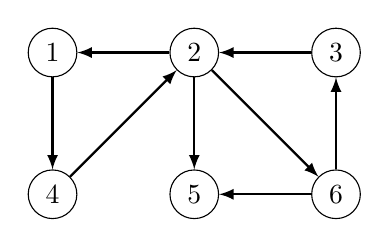
\begin{tikzpicture}[scale=0.9]
\node[draw, circle] (1) at (1,3) {$1$};
\node[draw, circle] (2) at (1,1) {$4$};
\node[draw, circle] (3) at (3,3) {$2$};
\node[draw, circle] (4) at (5,3) {$3$};
\node[draw, circle] (5) at (3,1) {$5$};
\node[draw, circle] (6) at (5,1) {$6$};

\path[draw,thick,->,>=latex] (1) -- (2);
\path[draw,thick,->,>=latex] (2) -- (3);
\path[draw,thick,->,>=latex] (3) -- (1);
\path[draw,thick,->,>=latex] (4) -- (3);
\path[draw,thick,->,>=latex] (3) -- (5);
\path[draw,thick,->,>=latex] (3) -- (6);
\path[draw,thick,->,>=latex] (6) -- (4);
\path[draw,thick,->,>=latex] (6) -- (5);
\end{tikzpicture}
\end{center}
ma trận kề là
\[
V= \begin{bmatrix}
  0 & 0 & 0 & 1 & 0 & 0 \\
  1 & 0 & 0 & 0 & 1 & 1 \\
  0 & 1 & 0 & 0 & 0 & 0 \\
  0 & 1 & 0 & 0 & 0 & 0 \\
  0 & 0 & 0 & 0 & 0 & 0 \\
  0 & 0 & 1 & 0 & 1 & 0 \\
 \end{bmatrix}.
\]
Bây giờ, ví dụ, ma trận
\[
V^4= \begin{bmatrix}
  0 & 0 & 1 & 1 & 1 & 0 \\
  2 & 0 & 0 & 0 & 2 & 2 \\
  0 & 2 & 0 & 0 & 0 & 0 \\
  0 & 2 & 0 & 0 & 0 & 0 \\
  0 & 0 & 0 & 0 & 0 & 0 \\
  0 & 0 & 1 & 1 & 1 & 0 \\
 \end{bmatrix}
\]
chứa số lượng đường đi có 4 cạnh
giữa các nút.
Ví dụ, $V^4[2,5]=2$,
bởi vì có hai đường đi 4 cạnh
từ nút 2 đến nút 5:
$2 \rightarrow 1 \rightarrow 4 \rightarrow 2 \rightarrow 5$
và
$2 \rightarrow 6 \rightarrow 3 \rightarrow 2 \rightarrow 5$.

\subsubsection{Đường đi ngắn nhất}

Sử dụng một ý tưởng tương tự trong đồ thị có trọng số,
ta có thể tính cho mỗi cặp nút độ dài nhỏ nhất
của đường đi 
giữa chúng có chính xác $n$ cạnh.
Để tính được điều này, ta phải định nghĩa phép nhân ma trận
theo một cách mới, sao cho ta không tính số lượng
đường đi mà tối thiểu hóa độ dài của đường đi.

\begin{samepage}
As an example, consider the following graph:
\begin{center}
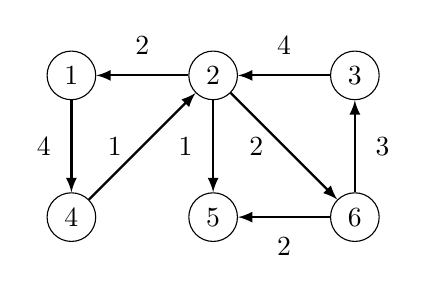
\begin{tikzpicture}[scale=0.9]
\node[draw, circle] (1) at (1,3) {$1$};
\node[draw, circle] (2) at (1,1) {$4$};
\node[draw, circle] (3) at (3,3) {$2$};
\node[draw, circle] (4) at (5,3) {$3$};
\node[draw, circle] (5) at (3,1) {$5$};
\node[draw, circle] (6) at (5,1) {$6$};

\path[draw,thick,->,>=latex] (1) -- node[font=\small,label=left:4] {} (2);
\path[draw,thick,->,>=latex] (2) -- node[font=\small,label=left:1] {} (3);
\path[draw,thick,->,>=latex] (3) -- node[font=\small,label=north:2] {} (1);
\path[draw,thick,->,>=latex] (4) -- node[font=\small,label=north:4] {} (3);
\path[draw,thick,->,>=latex] (3) -- node[font=\small,label=left:1] {} (5);
\path[draw,thick,->,>=latex] (3) -- node[font=\small,label=left:2] {} (6);
\path[draw,thick,->,>=latex] (6) -- node[font=\small,label=right:3] {} (4);
\path[draw,thick,->,>=latex] (6) -- node[font=\small,label=below:2] {} (5);
\end{tikzpicture}
\end{center}
\end{samepage}

Ta hãy xây dựng một ma trận kề trong đó
$\infty$ nghĩa là không tồn tại cạnh,
và các giá trị khác tương ứng với trọng số cạnh.
Ma trận là
\[
V= \begin{bmatrix}
  \infty & \infty & \infty & 4 & \infty & \infty \\
  2 & \infty & \infty & \infty & 1 & 2 \\
  \infty & 4 & \infty & \infty & \infty & \infty \\
  \infty & 1 & \infty & \infty & \infty & \infty \\
  \infty & \infty & \infty & \infty & \infty & \infty \\
  \infty & \infty & 3 & \infty & 2 & \infty \\
 \end{bmatrix}.
\]

Thay vì công thức
\[
AB[i,j] = \sum_{k=1}^n A[i,k] \cdot B[k,j]
\]
ta bây giờ sử dụng công thức
\[
AB[i,j] = \min_{k=1}^n A[i,k] + B[k,j]
\]
cho phép nhân ma trận, vì vậy ta tính
giá trị nhỏ nhất thay vì tổng,
và tổng các phần tử thay vì tích.
Sau sự thay đổi này,
lũy thừa ma trận tương ứng với
đường đi ngắn nhất trong đồ thị.

Ví dụ, khi
\[
V^4= \begin{bmatrix}
  \infty & \infty & 10 & 11 & 9 & \infty \\
  9 & \infty & \infty & \infty & 8 & 9 \\
  \infty & 11 & \infty & \infty & \infty & \infty \\
  \infty & 8 & \infty & \infty & \infty & \infty \\
  \infty & \infty & \infty & \infty & \infty & \infty \\
  \infty & \infty & 12 & 13 & 11 & \infty \\
 \end{bmatrix},
\]
ta có thể kết luận rằng độ dài nhỏ nhất của đường đi
có 4 cạnh
từ nút 2 đến nút 5 là 8.
Một đường đi như vậy là
$2 \rightarrow 1 \rightarrow 4 \rightarrow 2 \rightarrow 5$.

\subsubsection{Định lý Kirchhoff}

\index{Kirchhoff's theorem}
\index{định lý Kirchhoff}
\index{spanning tree}
\index{cây khung}

\key{Định lý Kirchhoff} (Kirchhoff's theorem)
%\footnote{G. R. Kirchhoff (1824--1887) was a German physicist.}
cung cấp một cách
để tính số lượng cây khung
của một đồ thị dưới dạng định thức của một ma trận đặc biệt.
Ví dụ, đồ thị
\begin{center}
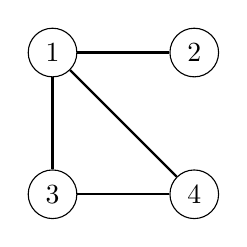
\begin{tikzpicture}[scale=0.9]
\node[draw, circle] (1) at (1,3) {$1$};
\node[draw, circle] (2) at (3,3) {$2$};
\node[draw, circle] (3) at (1,1) {$3$};
\node[draw, circle] (4) at (3,1) {$4$};

\path[draw,thick,-] (1) -- (2);
\path[draw,thick,-] (1) -- (3);
\path[draw,thick,-] (3) -- (4);
\path[draw,thick,-] (1) -- (4);
\end{tikzpicture}
\end{center}
has three spanning trees:
\begin{center}
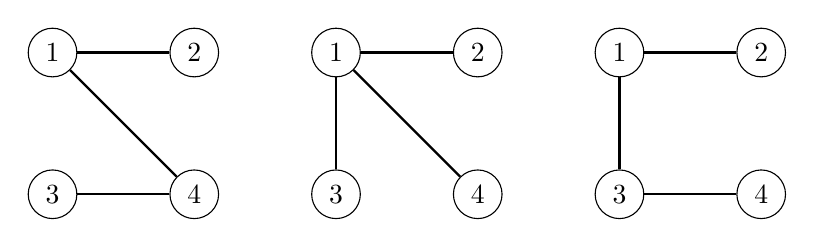
\begin{tikzpicture}[scale=0.9]
\node[draw, circle] (1a) at (1,3) {$1$};
\node[draw, circle] (2a) at (3,3) {$2$};
\node[draw, circle] (3a) at (1,1) {$3$};
\node[draw, circle] (4a) at (3,1) {$4$};

\path[draw,thick,-] (1a) -- (2a);
%\path[draw,thick,-] (1a) -- (3a);
\path[draw,thick,-] (3a) -- (4a);
\path[draw,thick,-] (1a) -- (4a);

\node[draw, circle] (1b) at (1+4,3) {$1$};
\node[draw, circle] (2b) at (3+4,3) {$2$};
\node[draw, circle] (3b) at (1+4,1) {$3$};
\node[draw, circle] (4b) at (3+4,1) {$4$};

\path[draw,thick,-] (1b) -- (2b);
\path[draw,thick,-] (1b) -- (3b);
%\path[draw,thick,-] (3b) -- (4b);
\path[draw,thick,-] (1b) -- (4b);

\node[draw, circle] (1c) at (1+8,3) {$1$};
\node[draw, circle] (2c) at (3+8,3) {$2$};
\node[draw, circle] (3c) at (1+8,1) {$3$};
\node[draw, circle] (4c) at (3+8,1) {$4$};

\path[draw,thick,-] (1c) -- (2c);
\path[draw,thick,-] (1c) -- (3c);
\path[draw,thick,-] (3c) -- (4c);
%\path[draw,thick,-] (1c) -- (4c);
\end{tikzpicture}
\end{center}
\index{Laplacean matrix}
\index{ma trận Laplace}
Để tính số lượng cây khung,
ta xây dựng một \key{ma trận Laplace} (Laplacean matrix) $L$,
trong đó $L[i,i]$ là bậc của nút $i$
và $L[i,j]=-1$ nếu có cạnh nối giữa
các nút $i$ và $j$, và ngược lại $L[i,j]=0$.
Ma trận Laplace cho đồ thị trên như sau:
\[
L= \begin{bmatrix}
  3 & -1 & -1 & -1 \\
  -1 & 1 & 0 & 0 \\
  -1 & 0 & 2 & -1 \\
  -1 & 0 & -1 & 2 \\
 \end{bmatrix}
\]

Có thể chứng minh rằng
số lượng cây khung bằng
định thức của ma trận thu được
khi ta loại bỏ bất kỳ hàng và cột nào từ $L$.
Ví dụ, nếu ta loại bỏ hàng
và cột đầu tiên, kết quả là

\[ \det(
\begin{bmatrix}
  1 & 0 & 0 \\
  0 & 2 & -1 \\
  0 & -1 & 2 \\
 \end{bmatrix}
) =3.\]
Định thức luôn giống nhau,
bất kể ta loại bỏ hàng và cột nào từ $L$.

Chú ý rằng công thức Cayley trong Chương 22.5 là
một trường hợp đặc biệt của định lý Kirchhoff,
bởi vì trong đồ thị đầy đủ có $n$ nút

\[ \det(
\begin{bmatrix}
  n-1 & -1 & \cdots & -1 \\
  -1 & n-1 & \cdots & -1 \\
  \vdots & \vdots & \ddots & \vdots \\
  -1 & -1 & \cdots & n-1 \\
 \end{bmatrix}
) =n^{n-2}.\]



